\documentclass[a4paper, 14pt]{extarticle}

% Поля
%----------------------
\usepackage{geometry}
\geometry{a4paper,left=2cm,right=1cm,
    top=2cm,bottom=2cm,bindingoffset=0cm}
%----------------------

% Russian-specific packages
%----------------------
\usepackage[T2A]{fontenc}
\usepackage[utf8]{inputenc}
\usepackage[english, main=russian]{babel}
%----------------------

\usepackage{textcomp}

% Красная строка
%----------------------
\usepackage{indentfirst}
%----------------------

% Graphics
%----------------------
\usepackage{graphicx}
\graphicspath{ {./images} }
\usepackage{wrapfig}
%----------------------

% Import minted
%----------------------
\usepackage{minted}
%----------------------

\linespread{1.3}
\sloppy
\clubpenalty=10000
\widowpenalty=10000

\begin{document}

%--------------------------------------
%			ТИТУЛЬНЫЙ ЛИСТ
%--------------------------------------
\begin{titlepage}
\thispagestyle{empty}
\newpage


%Шапка титульного листа
%--------------------------------------
\vspace*{-60pt}
\hspace{-65pt}
\begin{minipage}{0.3\textwidth}
\hspace*{-20pt}\centering

\includegraphics[width=\textwidth]{emblem}
\end{minipage}
\begin{minipage}{0.67\textwidth}\small \textbf{
\vspace*{-0.7ex}
\hspace*{-6pt}\centerline{Министерство науки и высшего образования Российской Федерации}
\vspace*{-0.7ex}
\centerline{Федеральное государственное бюджетное образовательное учреждение }
\vspace*{-0.7ex}
\centerline{высшего образования}
\vspace*{-0.7ex}
\centerline{<<Московский государственный технический университет}
\vspace*{-0.7ex}
\centerline{имени Н.Э. Баумана}
\vspace*{-0.7ex}
\centerline{(национальный исследовательский университет)>>}
\vspace*{-0.7ex}
\centerline{(МГТУ им. Н.Э. Баумана)}}
\end{minipage}
%--------------------------------------

%Полосы
%--------------------------------------
\vspace{-25pt}
\hspace{-35pt}\rule{\textwidth}{2.3pt}

\vspace*{-20.3pt}
\hspace{-35pt}\rule{\textwidth}{0.4pt}
%--------------------------------------

\vspace{1.5ex}
\hspace{-35pt} \noindent \small ФАКУЛЬТЕТ\hspace{80pt} <<Информатика и системы управления>>

\vspace*{-16pt}
\hspace{47pt}\rule{0.83\textwidth}{0.4pt}

\vspace{0.5ex}
\hspace{-35pt} \noindent \small КАФЕДРА\hspace{50pt} <<Теоретическая информатика и компьютерные технологии>>

\vspace*{-16pt}
\hspace{30pt}\rule{0.866\textwidth}{0.4pt}
  
\vspace{11em}

\begin{center}
\Large {\bf Лабораторная работа № 3} \\ 
\large {\bf по курсу <<Языки и методы программирования>>} \\
\large <<Полиморфизм на основе интерфейсов в языке Java>> \\
\large Вариант 15
\end{center}\normalsize

\vspace{8em}


\begin{flushright}
  {Студент группы ИУ9-22Б Павлов И. П. \hspace*{15pt}\\ 
  \vspace{2ex}
  Преподаватель Посевин Д. П.\hspace*{15pt}}
\end{flushright}

\bigskip

\vfill
 

\begin{center}
\textsl{Москва 2023}
\end{center}
\end{titlepage}
%--------------------------------------
%		КОНЕЦ ТИТУЛЬНОГО ЛИСТА
%--------------------------------------

\newpage
\section{Цель работы}
Приобретение навыков реализации интерфейсов для обеспечения возможности полиморфной обработки объектов класса.

\section{Условие}
Во время выполнения лабораторной работы требуется разработать на языке Java один из
классов, перечисленных в таблице. В классе должен быть реализован интерфейс Comparable<T>
и переопределён метод toString. В методе main вспомогательного класса Test нужно
продемонстрировать работоспособность разработанного класса путём сортировки массива его
экземпляров.

\section{Реализация основного класса}
{\scriptsize
\begin{minted}{java}
public class Main {
    public static void main(String[] args) {
        Board myBoard = new Board();
        Queen queen1 = new Queen(5, 5);
        Queen queen2 = new Queen(6, 6);
        Queen queen3 = new Queen(1, 7);

        myBoard.addQueen(queen1);
        myBoard.addQueen(queen2);
        myBoard.addQueen(queen3);

        System.out.println("Отсортированные ферзи (метод сортировки " +
                "внутри шахматной доски):");
        myBoard.getQueens();
    }
}
\end{minted}
}

\section{Реализация шахматной доски}
{\scriptsize
\begin{minted}{java}
import java.util.ArrayList;
import java.util.Collections;

import static java.lang.Math.abs;

public class Board {

    private ArrayList<Queen> queens = new ArrayList<>();
    private int elemCounter;

    private void countBeats() {
        for(int i = 0; i < this.elemCounter; i++) {
            Queen queen1 = this.queens.get(i);
            int x1 = queen1.getX();
            int y1 = queen1.getY();

            for (int j = i; j < this.elemCounter; j++) {
                Queen queen2 = this.queens.get(j);
                int x2 = queen2.getX();
                int y2 = queen2.getY();
                if (x1 == x2 || y1 == y2 || abs(x1 - x2) == abs(y1 - y2)) {
                    queen1.setBeatCounter(queen1.getBeatCounter() + 1);
                    queen2.setBeatCounter(queen2.getBeatCounter() + 1);
                }
            }
        }
    }


    public void addQueen(Queen entity) {
        this.queens.add(entity);
        this.elemCounter++;
    }

    public void getQueens() {
        countBeats();
        Collections.sort(this.queens);
        for(int i = 0; i < this.elemCounter; i++) {
            System.out.println(this.queens.get(i));
        }
    }

}
\end{minted}
}

\section{Реализация ферзя}
{\scriptsize
\begin{minted}{java}
public class Queen implements Comparable<Queen> {

    private final int x;
    private final int y;
    private int beatCounter;

    public Queen(int x, int y) {
        this.x = x;
        this.y = y;
        this.beatCounter = 0;
    }

    public int getX() {
        return x;
    }

    public int getY() {
        return y;
    }

    public int getBeatCounter() {
        return this.beatCounter;
    }

    public void setBeatCounter(int x) {
        this.beatCounter = x;
    }

    public int compareTo(Queen entity) {
        return Integer.compare(this.beatCounter, entity.getBeatCounter());
    }

    public String toString() {
        return "Координаты ферзя: (" + this.x + ", " + this.y + "). Бьёт "
                + this.beatCounter + " ферзей";
    }
}
\end{minted}
}

\begin{figure}[h] 
\center{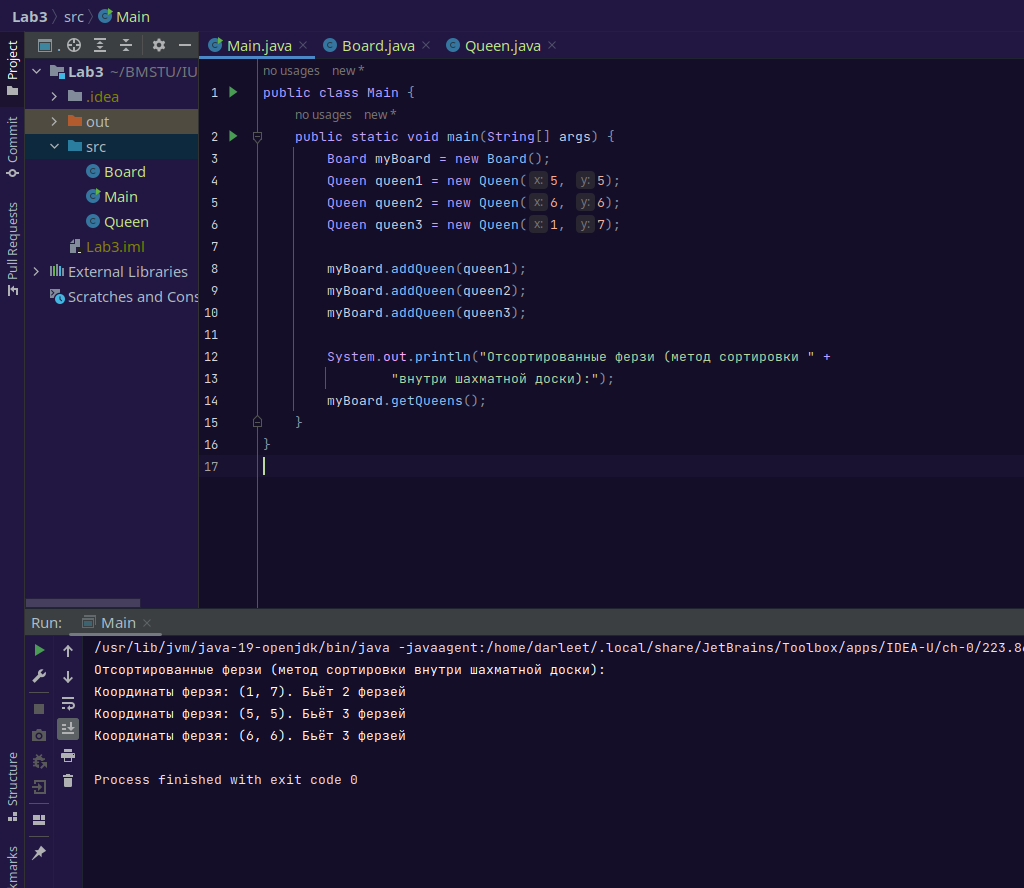
\includegraphics[scale=0.45]{class_main.png}} 
\caption{Вывод программы} 
\label{fig:image} 
\end{figure}

\end{document}
